%%%%%%%%%%%%%%%%%%%%%%%%%%%%%%%%%%%%
% Slide options
%%%%%%%%%%%%%%%%%%%%%%%%%%%%%%%%%%%%

% Option 1: Slides with solutions

\documentclass[slidestop,compress,mathserif]{beamer}
\newcommand{\soln}[1]{\textit{#1}}
\newcommand{\solnGr}[1]{#1}

% Option 2: Handouts without solutions

%\documentclass[11pt,containsverbatim,handout]{beamer}
%\usepackage{pgfpages}
%\pgfpagesuselayout{4 on 1}[letterpaper,landscape,border shrink=5mm]
%\newcommand{\soln}[1]{ }
%\newcommand{\solnGr}{ }

%%%%%%%%%%%%%%%%%%%%%%%%%%%%%%%%%%%%
% Style
%%%%%%%%%%%%%%%%%%%%%%%%%%%%%%%%%%%%

\def\chp8@path{../../Chp 8}
\input{../../lec_style.tex}

%%%%%%%%%%%%%%%%%%%%%%%%%%%%%%%%%%%%
% Preamble
%%%%%%%%%%%%%%%%%%%%%%%%%%%%%%%%%%%%

\title[Lecture 35]{MA213: Lecture 35}
\subtitle{Module 5: Linear regression}
\author{OpenIntro Statistics, 4th Edition}
\institute{$\:$ \\ {\footnotesize Based on slides developed by Mine \c{C}etinkaya-Rundel of OpenIntro. \\
The slides may be copied, edited, and/or shared via the \webLink{http://creativecommons.org/licenses/by-sa/3.0/us/}{CC BY-SA license.} \\
Some images may be included under fair use guidelines (educational purposes).}}
\date{}


%%%%%%%%%%%%%%%%%%%%%%%%%%%%%%%%%%%%
% Begin document
%%%%%%%%%%%%%%%%%%%%%%%%%%%%%%%%%%%%

\begin{document}


%%%%%%%%%%%%%%%%%%%%%%%%%%%%%%%%%%%%
% Title page
%%%%%%%%%%%%%%%%%%%%%%%%%%%%%%%%%%%%

{
\addtocounter{framenumber}{-1} 
{\removepagenumbers 
\usebackgroundtemplate{\includegraphics[width=\paperwidth]{../../OpenIntro_Grid_4_3-01.jpg}}
\begin{frame}

\hfill \includegraphics[width=20mm]{../../oiLogo_highres}

\titlepage

\end{frame}
}
}


%%%%%%%%%%%%%%%%%%%%%%%%%%%%%%%%%%%%
% Recap/Agenda 
%%%%%%%%%%%%%%%%%%%%%%%%%%%%%%%%%%%%
% TODO better formatting
\begin{frame}
    \frametitle{Module 5: Linear regression}
    \begin{itemize}
        \item \hl{Previously: }Types of outliers in linear regression (Chapter 8.3)
        \item \hl{This time: }Inference for linear regression (Chapter 8.4)
        \item \hl{Reading: }Chapter 8.4 for next time
        \item \hl{Deadlines/Announcements: }HW 5.1 due today, Q4 in discussions this week
    \end{itemize}
    
\end{frame}
%%%%%%%%%%%%%%%%%%%%%%%%%%%%%%%%%%%%
% Sections
%%%%%%%%%%%%%%%%%%%%%%%%%%%%%%%%%%%%

%%%%%%%%%%%%%%%%%%%%%%%%%%%%%%%%%%%%

\section{Inferece for linear regression, continued}

%%%%%%%%%%%%%%%%%%%%%%%%%%%%%%%%%%%%

\begin{frame}
    \frametitle{Last time: $t$-test for the slope}
\end{frame}


\begin{frame}
\frametitle{\% College graduate vs. \% Hispanic in LA}

\dq{What can you say about the relationship between \% college graduate and \% Hispanic in a sample of 100 zip code areas in LA?}

\begin{center}
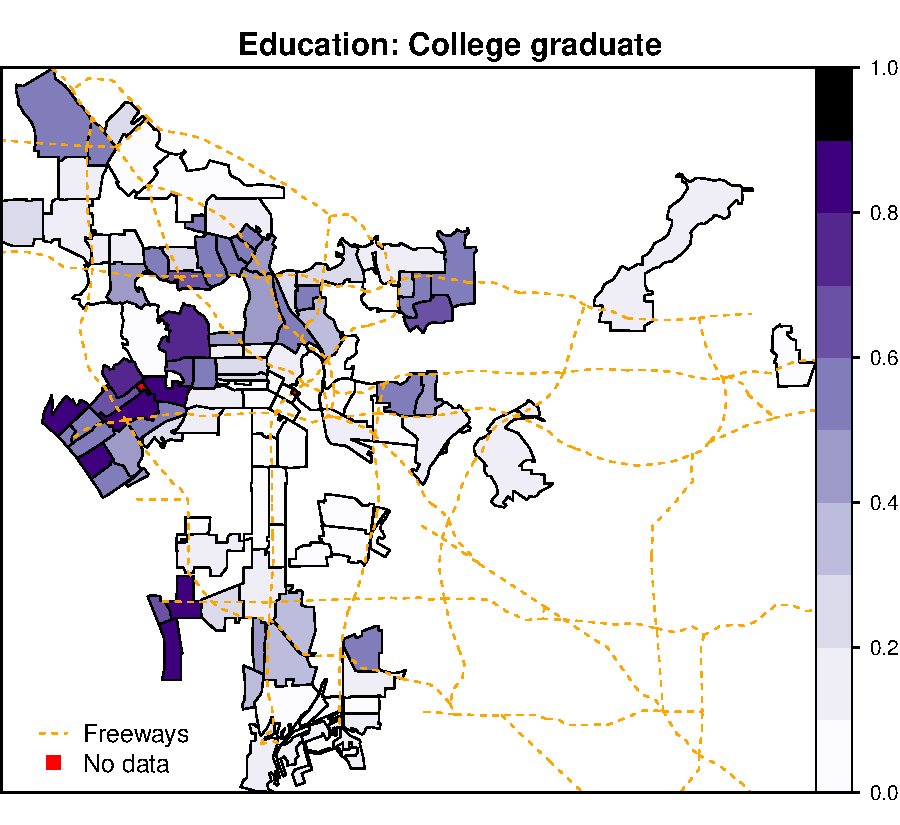
\includegraphics[width=0.49\textwidth]{\chp8@path/8-4_inf_lin_reg/figures/la/Prop_EduHigherThan16th}~~~~
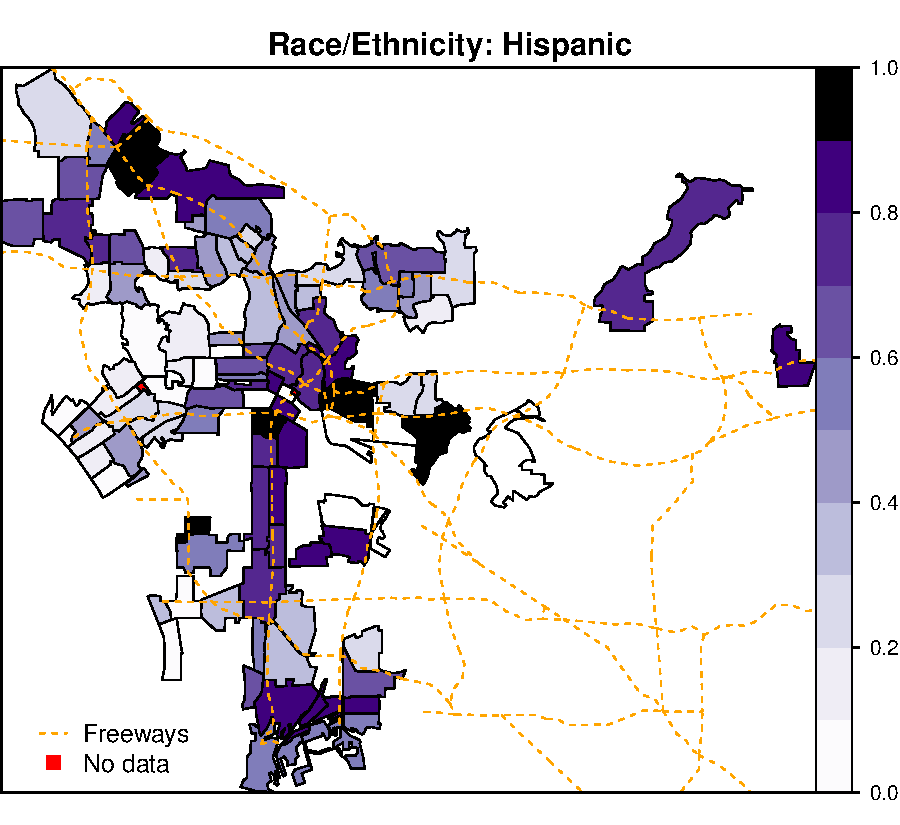
\includegraphics[width=0.49\textwidth]{\chp8@path/8-4_inf_lin_reg/figures/la/Prop_RaceEthHispanic}
\end{center}

\end{frame}

%%%%%%%%%%%%%%%%%%%%%%%%%%%%%%%%%%%

\begin{frame}
\frametitle{\% College educated vs. \% Hispanic in LA - another look}

\dq{What can you say about the relationship between of \% college graduate and \% Hispanic in a sample of 100 zip code areas in LA?}

\begin{center}
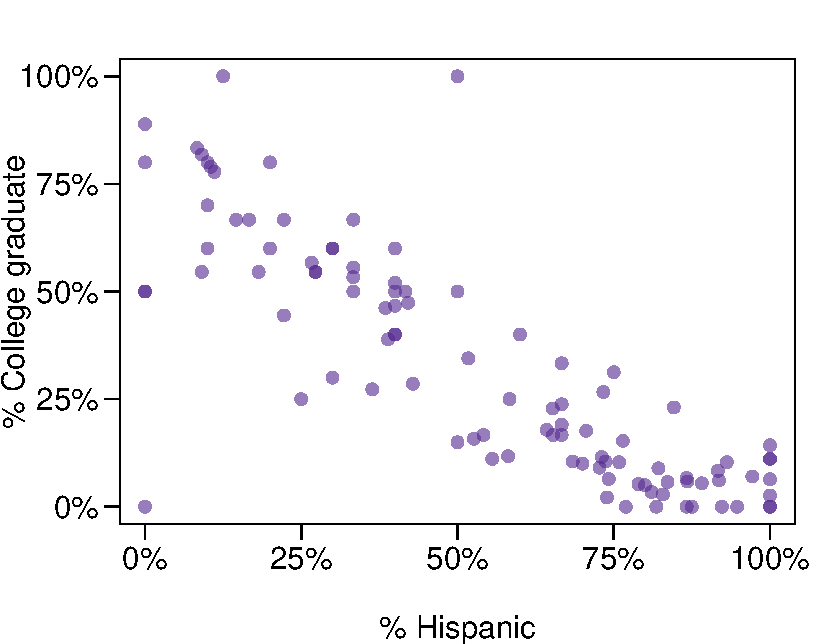
\includegraphics[width=0.7\textwidth]{\chp8@path/8-4_inf_lin_reg/figures/la/la}
\end{center}

\end{frame}

%%%%%%%%%%%%%%%%%%%%%%%%%%%%%%%%%%%

\begin{frame}
\frametitle{\% College educated vs. \% Hispanic in LA - linear model}

\pq{Which of the below is the best interpretation of the slope?}

{\small
\begin{center}
\begin{tabular}{rrrrr}
  \hline
 & Estimate & Std. Error & t value & Pr($>$$|$t$|$) \\ 
  \hline
(Intercept) & 0.7290 & 0.0308 & 23.68 & 0.0000 \\ 
 \%Hispanic & -0.7527 & 0.0501 & -15.01 & 0.0000 \\ 
   \hline
%   &&&&$df$ = 98 \\
\end{tabular}
\end{center}
}

\begin{enumerate}[(a)]
\item A 1\% increase in Hispanic residents in a zip code area in LA is associated with a 75\% decrease in \% of college grads.
\solnMult{A 1\% increase in Hispanic residents in a zip code area in LA is associated with a 0.75\% decrease in \% of college grads.}
\item An additional 1\% of Hispanic residents decreases the \% of college graduates in a zip code area in LA by 0.75\%.
\item In zip code areas with no Hispanic residents, \% of college graduates is expected to be 75\%.
\end{enumerate}

\end{frame}

%%%%%%%%%%%%%%%%%%%%%%%%%%%%%%%%%%%

\begin{frame}
\frametitle{\% College educated vs. \% Hispanic in LA - linear model}

\dq{Do these data provide convincing evidence that there is a statistically significant relationship between \% Hispanic and \% college graduates in zip code areas in LA?}

{\small
\begin{center}
\begin{tabular}{rrrrr}
  \hline
 & Estimate & Std. Error & t value & Pr($>$$|$t$|$) \\ 
  \hline
(Intercept) & 0.7290 & 0.0308 & 23.68 & 0.0000 \\ 
  hispanic & -0.7527 & 0.0501 & -15.01 & 0.0000 \\ 
   \hline
%   &&&&$df$ = 98 \\
\end{tabular}
\end{center}
}
\soln{\only<2->{Yes, the p-value for \% Hispanic is low, indicating that the data provide convincing evidence that the slope parameter is different than 0.
}}

$\:$ \\

\dq{How reliable is this p-value if these zip code areas are not randomly selected?}
\soln{\only<3->{Not very...
}}

\end{frame}

%%%%%%%%%%%%%%%%%%%%%%%%%%%%%%%%%%%

\section{R Demonstration: CI for the slope}

%%%%%%%%%%%%%%%%%%%%%%%%%%%%%%%%%%%

\section{Edfinity Quiz: CI for the slope}

%%%%%%%%%%%%%%%%%%%%%%%%%%%%%%%%%%%

\subsection{CI for the slope}

%%%%%%%%%%%%%%%%%%%%%%%%%%%%%%%%%%%

\begin{frame}
\frametitle{Confidence interval for the slope}

\pq{{\small Remember that a confidence interval is calculated as $point~estimate \pm ME$ and the degrees of freedom associated with the slope in a simple linear regression is $n - 2$. Which of the below is the correct 95\% confidence interval for the slope parameter? Note that the model is based on observations from 27 twins.}}

{\footnotesize
\begin{center}
\begin{tabular}{rrrrr}
  \hline
 & Estimate & Std. Error & t value & Pr($>$$|$t$|$) \\ 
  \hline
(Intercept) & 9.2076 & 9.2999 & 0.99 & 0.3316 \\ 
  bioIQ & 0.9014 & 0.0963 & 9.36 & 0.0000 \\ 
   \hline
\end{tabular}
\end{center}
}

\vspace{-0.5cm}

\twocol{0.4}{0.6}
{
\begin{enumerate}[(a)]
\item $9.2076 \pm 1.65 \times 9.2999$
\solnMult{ $0.9014 \pm 2.06 \times 0.0963$}
\item $0.9014 \pm 1.96 \times 0.0963$
\item $9.2076 \pm 1.96 \times 0.0963$
\end{enumerate}
}
{
\soln{\onslide<2->{\orange{
\begin{eqnarray*}
\pause
n &=& 27 \qquad df = 27 - 2 = 25 \\
\pause
95\%:~t^\star_{25} &=& 2.06 \\
\pause
0.9014 &\pm& 2.06 \times 0.0963 \\
\pause
(0.7 &,& 1.1)
\end{eqnarray*}
}}}}

\end{frame}

%%%%%%%%%%%%%%%%%%%%%%%%%%%%%%%%%%%

\begin{frame}
\frametitle{Recap}

\begin{itemize}

\item Inference for the slope for a single-predictor linear regression model:
\pause
\begin{itemize}
\item Hypothesis test:
\[ T = \frac{b_1 - null~value}{SE_{b_1}} \qquad df = n - 2 \]
\pause
\item Confidence interval:
\[ b_1 \pm t^\star_{df = n - 2} SE_{b_1} \]
\end{itemize}

\pause

\item The null value is often 0 since we are usually checking for \hl{any} relationship between the explanatory and the response variable.

\pause

\item The regression output gives $b_1$, $SE_{b_1}$, and \hl{two-tailed} p-value for the $t$-test for the slope where the null value is 0.

\pause

\item We rarely do inference on the intercept, so we'll be focusing on the estimates and inference for the slope.

\end{itemize}

\end{frame}

%%%%%%%%%%%%%%%%%%%%%%%%%%%%%%%%%%%


\begin{frame}
\frametitle{Caution}

\begin{itemize}

\item Always be aware of the type of data you're working with: random sample, non-random sample, or population.

\pause

\item Statistical inference, and the resulting p-values, are meaningless when you already have population data.

\pause

\item If you have a sample that is non-random (biased), inference on the results will be unreliable.

\pause

\item The ultimate goal is to have independent observations.

\end{itemize}

\end{frame}

%%%%%%%%%%%%%%%%%%%%%%%%%%%%%%%%%%%

%%%%%%%%%%%%%%%%%%%%%%%%%%%%%%%%%%%%
% End document
%%%%%%%%%%%%%%%%%%%%%%%%%%%%%%%%%%%%

\end{document}